\documentclass[10pt,a4paper]{article}
\usepackage[utf8]{inputenc}
\usepackage[T1]{fontenc}
\usepackage[czech]{babel}
\usepackage[tmargin=1in,bmargin=1in,lmargin=1in,rmargin=1in]{geometry}
\usepackage{times}
\usepackage[none]{hyphenat}
\usepackage{graphicx}
% \usepackage[unicode, colorlinks, hypertexnames=false, citecolor=red]{hyperref}

\renewcommand{\baselinestretch}{1.2}

\begin{document}
    {\noindent\sffamily\large
        \textbf{Implementační dokumentace k 2. úloze do IPP 2020/2021} \\
        Jméno a~příjmení: Petr Kabelka \\
        Login: xkabel09
    }

    \section{Interpret}

    Skript \emph{interpret.py} je rozdělen do několika tříd které mají na starosti
    jednotlivé části interpretu. Vztahy mezi jednotlivými třídami jsou znázorněny na následujícím diagramu.

    \begin{figure}[ht]
        \centering
        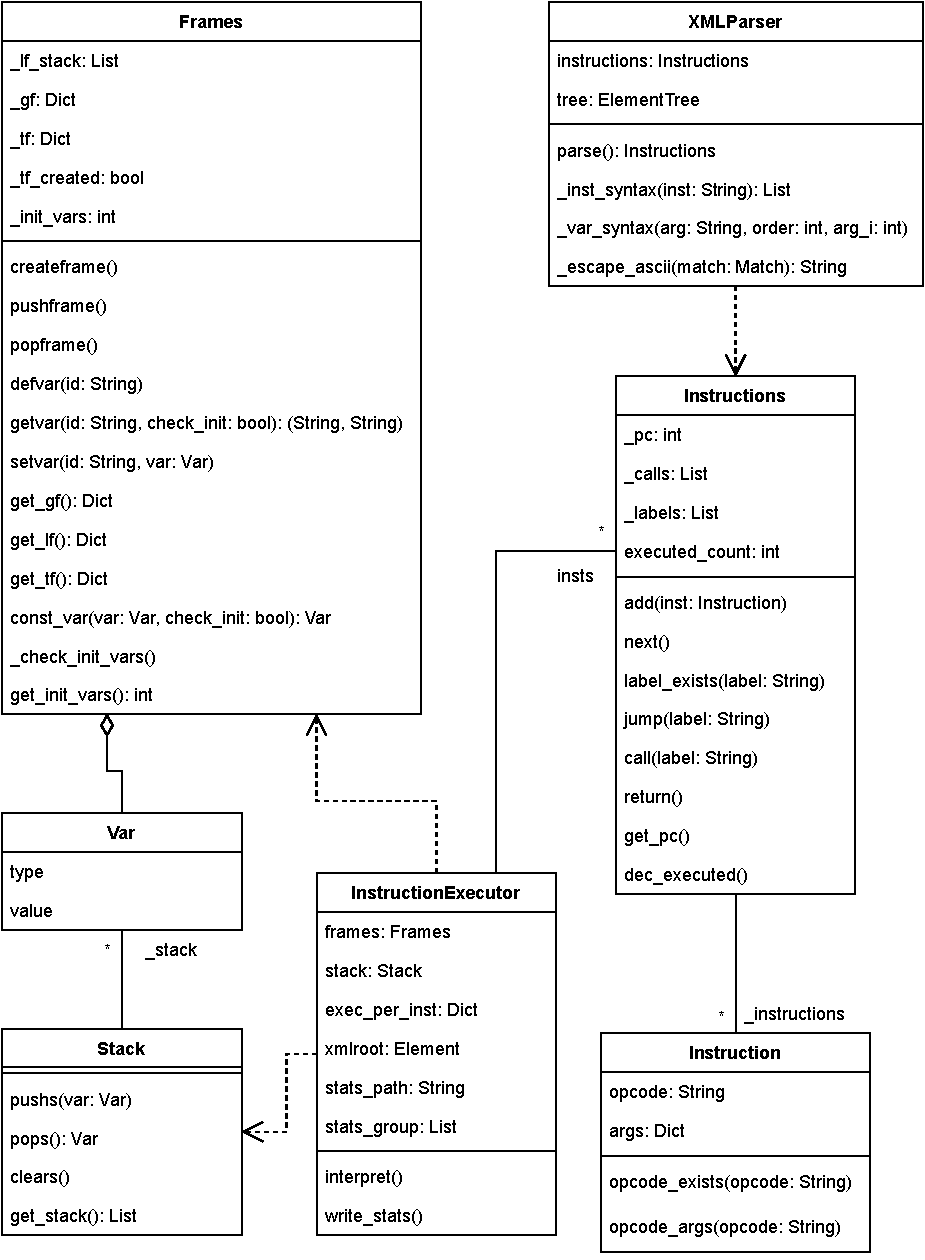
\includegraphics[width=13cm]{interpret-class-diagram.pdf}
        \caption{Diagram tříd interpretu}
    \end{figure}

    Vše začíná třídou \emph{XMLParser} a~její metodou \emph{parse}, která provede
    nad zdrojovým kódem v~XML lexikální a~syntaktickou analýzu podobně jako ve
    skriptu \emph{parse.php}. Proměnná \emph{\_INST\_MAP} mapuje operační kód instrukce
    na typy operandů, které příjímá. Zpracované instrukce po analýze kódu předáme třídě
    \emph{InstructionExecutor}, která řídí hlavní činnost interpretu.

    InstructionExecutor si nejprve vytvoří instance všech potřebných tříd a~po
    zavolání metody \emph{interpret} začne vykonávat instrukce v~cyklu dokud jsou
    nějaké na instrukční pásce. Každá instrukce má implementovanou svoji metodu která vykonává její činnost.
    Tyto metody začínají znakem podtržítka za kterým následuje operační kód instrukce.
    Díky tomuto formátu je možné volat funkcí \emph{eval} příslušné metody spolu
    s~argumenty instrukce. Sběr a~zápis statistik jsem zabudoval do třídy InstructionExecutor, neboť
    ovládá všechny části interpretu a~má přehled o~všech sbíraných údajích.

    Většina metod pro instrukce jednoduše získá vstupní operandy a~provede
    odpovídající operaci mezi těmito proměnnými, které jsou instancemi třídy \emph{Var},
    ta implementuje magické metody pro všechny potřebné operace.

    Při implementaci chování interpretu v~různých krajních případech či způsobem
    výpisu výstupu z~ladících instrukcí jsem se řídil podle interpretu \emph{ic20int}.

    \subsection{Rozšíření}

    V~rámci řešení 2.~projektu jsem implementoval rozšíření \textbf{STATI},
    umožňující sběr statistik o~vykonávaném kódu, \textbf{FLOAT} pro práci s~datovým
    typem float a~také \textbf{STACK} umožňující používat zásobníkové varianty
    vybraných instrukcí.

    \section{Testovaní skript}

    Skript \emph{test.php} kontroluje přítomnost potřebných souborů a~složek
    s~ohledem na zvolené přepínače. Například není potřeba kontrolovat přítomnost
    interpretu při použití přepínače\verb| --parse-only|.

    Pro procházení složek rekurzivně je použita kombinace třídy \emph{RecursiveDirectoryIterator}
    a~dalších iterátorů. Pro procházení jedné složky pak stačí jen funkce \emph{scandir}.
    Skript si připraví tři dočasné soubory pro zapisování výstupů z~testů které následně spustí.
    Výsledky sbírá do asociativního pole, kde klíči jsou cesty k~testům bez přípon.
    Po spuštění všech testů se sestaví a~vypíše na standardní výstup
    jednoduchá HTML tabulka s~barevnými řádky -- zelené řádky indikují úspěšný test; červené řádky indikují neúspěšný test.

    Testovací skript mi velice pomohl při odhalení chyb které nebyly na první pohled viditelné.

\end{document}
